\section{Overview}
Figure~\ref{fig:overview} shows the different parts of Plan Merging: Individual Pathfinding, Path Selection and Solving.

\begin{figure}[H]
    \centering
    \caption{Overview of the thesis}\label{fig:overview}
    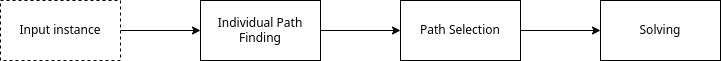
\includegraphics[width=\widthimg]{img/overview.drawio.png}
\end{figure}

Plan Merging involves processing multiple paths for each agents. These paths can be computed with Individual Path Finding~\ref{sec:ipf}. IPF can be a constituent of Plan Merging but we can define Plan Merging without the IPF part.

The second step of Plan Merging is Path Selection~\ref{sec:pathselection}. Path Selection has the goal of identifying paths that closely resemble valid solutions to the problem. However, it necessitates the construction of conflict-free set of path, which is computationally intensive, especially with a lot of agents and many paths. This is where we incorporate Path Elimination to reduce the number of paths by eliminating potentially ``problematic'' paths using a conflict-based strategy.

The final stage of Plan Merging involves obtaining a solution. We utilize the pre-computed paths provided by Path Selection, by using the paths in their original form, or by employing the delineation of the pre-computed paths as a subgraph in order to reduce the map size.




